% Arystal engine v1 — architecture and design rationale
% Build: tectonic engine_architecture.tex   (or latexmk -pdf)
% Figures: python make_figures.py  (data from docs/regime_study.md)
\documentclass[11pt,a4paper]{article}
\usepackage[T1]{fontenc}
\usepackage[utf8]{inputenc}
\usepackage{mathpazo}
\usepackage[final]{microtype}
\usepackage[a4paper,margin=27mm,top=25mm]{geometry}
\usepackage{amsmath}
\usepackage{siunitx}
\sisetup{per-mode=symbol, inter-unit-product=\ensuremath{{}\cdot{}}}
\usepackage{booktabs}
\usepackage{tabularx}
\usepackage{graphicx}
\usepackage[font=small,labelfont=bf,skip=4pt]{caption}
\usepackage{enumitem}
\usepackage[hyphens]{url}
\usepackage[hidelinks]{hyperref}
\usepackage[numbers,sort&compress]{natbib}
\usepackage{fancyhdr}
\usepackage{xcolor}
\usepackage{listings}
\lstset{basicstyle=\ttfamily\small, columns=fullflexible, keepspaces=true,
  frame=lines, framerule=0.3pt, aboveskip=8pt, belowskip=8pt,
  showstringspaces=false, breaklines=true, xleftmargin=1.2em,
  commentstyle=\itshape\color{black!60}, keywordstyle=\bfseries,
  language=Python}
\usepackage{tikz}
\usetikzlibrary{positioning,arrows.meta}
\pagestyle{fancy}\fancyhf{}
\renewcommand{\headrulewidth}{0pt}
\fancyfoot[C]{\small\thepage}
\setlength{\parindent}{1.2em}
\setlength{\parskip}{0pt}
\frenchspacing
\clubpenalty=10000 \widowpenalty=10000
\usepackage[htt]{hyphenat}
\newcommand{\code}[1]{\texttt{#1}}
\emergencystretch=2.5em

\makeatletter
\renewcommand{\maketitle}{%
  \begin{center}
    {\small\scshape \@context\par}\vspace{6pt}
    {\LARGE \@title\par}\vspace{6pt}
    {\normalsize \@author\par}
  \end{center}\vspace{10pt}}
\newcommand{\context}[1]{\gdef\@context{#1}}
\makeatother

\title{The Arystal Engine: Architecture and Design Rationale}
\context{Arystal engine v1 (Phase 1) \quad$\cdot$\quad November 2026}
\author{Luna F.}

\begin{document}
\maketitle

\noindent Arystal simulates the growth of an amethyst crystal ($\alpha$-quartz with trace iron) from the wall of a geode cavity into a low-temperature hydrothermal fluid. Version~1 is a two-dimensional phase-field engine written in Python, run on a single laptop CPU. The section modelled is longitudinal: it contains the crystal's $c$-axis, so it shows the prism and the pointed rhombohedral termination. This note is for a developer or a physicist joining the project. It explains what the engine computes, how the code is divided, how one simulation flows through it, and why the main decisions were taken. It does not replace the step-by-step instructions in \code{docs/how\_to\_run.md} or the per-function listing in \code{docs/function\_map.md}.

\tableofcontents

%======================================================================
\section{The physical model in brief}\label{sec:model}

The engine evolves four fields on a regular grid: the phase field $\phi$ ($\phi=1$ in the crystal, $0$ in the fluid, smooth across an interface a few cells wide), the dissolved silica $c$ (\si{\mole\per\kilo\gram}), the dissolved iron $f$, and the iron locked in the crystal $I$. All quantities inside the engine are non-dimensional (lengths in cells, time in model units); conversion to physical units happens outside the time step (Section~\ref{sec:time}).

\paragraph{Interface motion.} The phase field obeys an Allen--Cahn equation with a tilted double well,
\begin{equation}\label{eq:phasefield}
  \frac{\tau}{g(\theta)}\,\frac{\partial\phi}{\partial t}
  = \epsilon^{2}\nabla^{2}\phi + \phi(1-\phi)\left(\phi-\tfrac12+m\right),
\end{equation}
where $\tau$ is a relaxation time, $\epsilon$ sets the interface width (about one cell; the 10--90\,\% width is about $6.2\epsilon$), and $g(\theta)$ is the kinetic anisotropy factor discussed below. The tilt $m$ is the driving force for growth. It is computed from the supersaturation $S=c/c_\mathrm{eq}(T)$ as
\begin{equation}\label{eq:driving}
  m = \lambda \ln\frac{c}{c_\mathrm{eq}(T)}, \qquad |m|\le m_\mathrm{max}=0.3 ,
\end{equation}
with a kinetic coupling $\lambda=0.2$. The clip keeps $|m|$ below $1/2$, beyond which the fluid state $\phi=0$ would become unstable. With $m$ constant and no anisotropy, Eq.~\eqref{eq:phasefield} has the exact flat-front speed $v=\sqrt2\,\epsilon m/\tau$; validation check~1 reproduces it to \SI{0.73}{\percent}.

\paragraph{Solubility.} The equilibrium concentration follows the quartz curve of \citet{Rimstidt1997}, as printed in \citet{Takeno2000},
\begin{equation}\label{eq:solubility}
  \log_{10} c_\mathrm{eq} = \frac{A}{T} + B,\qquad A=\SI{-1107.12}{\kelvin},\quad B=-0.0254,
\end{equation}
with $c_\mathrm{eq}$ in \si{\mole\per\kilo\gram} and $T$ in kelvin. At \SI{25}{\celsius} it gives \SI{1.83e-4}{\mole\per\kilo\gram}, or \SI{10.97}{ppm} SiO$_2$, consistent with the $11.0\pm1.1$\,ppm usually quoted for Rimstidt's value at that temperature. The fluid starts saturated at a chosen higher temperature (default \SI{60}{\celsius}); running at a lower temperature therefore makes it supersaturated.

\paragraph{Silica transport.} Silica diffuses through the fluid only, and every unit of fluid that becomes crystal takes $C_\mathrm{s}$ of silica out of solution:
\begin{equation}\label{eq:silica}
  \frac{\partial c}{\partial t} = \nabla\cdot\big[D\,(1-h(\phi))\,\nabla c\big] - C_\mathrm{s}\,\frac{\partial h(\phi)}{\partial t},
  \qquad h(\phi)=\phi^{2}(3-2\phi).
\end{equation}
Diffusion is written as exchanges across cell faces with no flux at the container walls, so the total $\sum(c+C_\mathrm{s}h)$ is conserved to round-off. Validation check~3 measures a drift of order $10^{-14}$.

\paragraph{Faceting.} Quartz grows with flat faces. In the chosen section the prism faces $m$ are vertical, and the rhombohedral faces $r\{10\bar11\}$ and $z\{01\bar11\}$ form the termination, $r$ on one side and $z$ on the other. The angle between the $r$ pole and the $c$-axis, \SI{51.78}{\degree}, follows from the lattice parameters. The engine imposes a normal growth speed for each face family and builds the speed-versus-orientation function $g(\theta)$ from them (Frank's kinetic Wulff construction): $g$ is the support function of the polygon bounded by the half-planes $\mathbf n_k\cdot\mathbf x\le v_k$, with its cusps rounded by a log-sum-exp of sharpness $\beta=40$. Slow orientations survive as flat faces; fast ones grow out. The speeds are $v_m:v_r:v_z=0.5:1:1$.

\paragraph{Iron and colour.} Iron is a passive trace. It diffuses like silica and is incorporated where the crystal grows, with a molar distribution coefficient $k$ that depends on the local growth sector:
\begin{equation}\label{eq:iron}
  \mathrm dI = k(\text{sector})\,\frac{f}{c}\,C_\mathrm{s}\,\mathrm dh \quad(\mathrm dh>0),
  \qquad
  \mathrm dI = I\,\frac{\mathrm dh}{h}\quad(\mathrm dh<0).
\end{equation}
The coefficients are $k_r=0.01$, $k_z=0.005$, $k_m=0.001$, blended between sectors by a Gaussian of width \SI{12}{\degree} in the surface-normal direction. Colour is rendered from the crystal Fe/Si ratio through a saturating law; iron alone does not make amethyst (irradiation is also needed \citep{Cohen1974}), so the colour law assumes a uniform, sufficient dose.

\paragraph{Noise.} A multiplicative term $\sigma\sqrt{\Delta t/\tau}\,4\phi(1-\phi)\,\xi$, with $\xi$ standard normal and $\sigma=0.02$, acts only at the interface. The $\sqrt{1/\tau}$ factor keeps it in proportion to the deterministic dynamics; an early version without it roughened the surface when $\tau$ was large. Together with small random variations of the initial seed (\SI{5}{\percent} in radius, one cell in position), it is the only source of difference between replicas.

\paragraph{What is imposed and what is predicted.} Table~\ref{tab:imposed} separates the two. A reader should not take any simulated habit or colour contrast as a prediction about real amethyst: both follow from imposed inputs that no source has yet constrained quantitatively.

\begin{table}[ht]
\caption{Inputs imposed by assumption and outputs the model predicts from them. Status labels follow \code{materials/amethyst.yaml}.}\label{tab:imposed}
\small
\begin{tabularx}{\textwidth}{@{}lX@{}}
\toprule
Imposed (\textsc{assumed}) & Face speeds $v_m:v_r:v_z$ and hence the habit; $r=z$ in the section; iron coefficients (only the order $r>z>m$ has qualitative support); colour law; fluid iron \SI{1}{ppm}; noise and seed-variation amplitudes; $C_\mathrm{s}$; $\lambda$; closed container. \\
\addlinespace
Predicted & Position and orientation of flat faces; the sector pattern of iron; enrichment of surface Fe/Si where silica is depleted; conservation; response to temperature and iron changes; dependence of shape on Da and its plateau. \\
\addlinespace
Not predicted & The real habit of geode amethyst, its colour intensity, its growth time. \\
\bottomrule
\end{tabularx}
\end{table}

%======================================================================
\section{How the code is organised}\label{sec:layout}

The package \code{arystal/} is divided by responsibility, and dependencies point in one direction only (Figure~\ref{fig:layers}). The \code{engine} knows only physics: it reads no files, opens no windows and creates no random numbers. The \code{simulation} layer configures and drives runs. The \code{server} drives the simulation layer and nothing imports the server. Table~\ref{tab:folders} lists each folder.

\begin{figure}[ht]
\centering
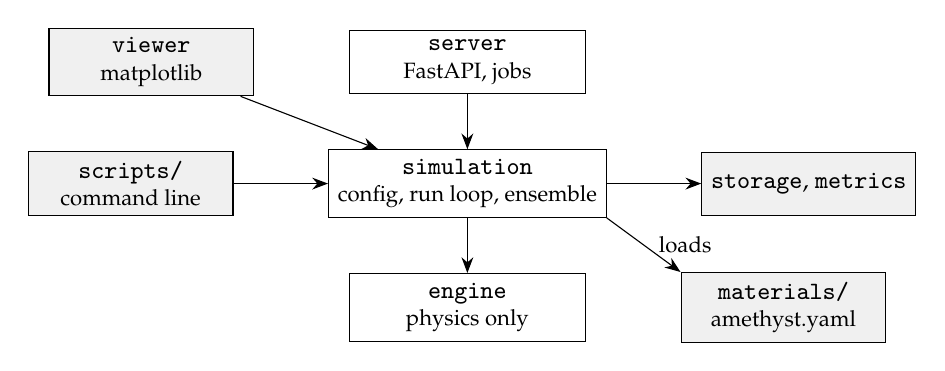
\begin{tikzpicture}[
  box/.style={draw, rectangle, minimum width=30mm, minimum height=8mm, align=center, font=\small},
  side/.style={draw, rectangle, minimum width=26mm, minimum height=8mm, align=center, font=\small, fill=black!6},
  arr/.style={-{Stealth[length=2mm]}, thin},
  node distance=7mm and 12mm]
\node[box] (server) {\code{server}\\[-1pt]{\footnotesize FastAPI, jobs}};
\node[box, below=of server] (sim) {\code{simulation}\\[-1pt]{\footnotesize config, run loop, ensemble}};
\node[box, below=of sim] (engine) {\code{engine}\\[-1pt]{\footnotesize physics only}};
\node[side, left=of server] (viewer) {\code{viewer}\\[-1pt]{\footnotesize matplotlib}};
\node[side, left=of sim] (scripts) {\code{scripts/}\\[-1pt]{\footnotesize command line}};
\node[side, right=of sim] (storage) {\code{storage}, \code{metrics}};
\node[side, right=of engine] (yaml) {\code{materials/}\\[-1pt]{\footnotesize amethyst.yaml}};
\draw[arr] (server) -- (sim);
\draw[arr] (sim) -- (engine);
\draw[arr] (viewer) -- (sim);
\draw[arr] (scripts) -- (sim);
\draw[arr] (sim) -- (storage);
\draw[arr] (sim.south east) -- node[right=2pt, font=\footnotesize]{loads} (yaml.north west);
\end{tikzpicture}
\caption{Layers of the engine. An arrow means ``uses''. Shaded boxes are clients or support modules; none of them is imported by \code{engine}.}\label{fig:layers}
\end{figure}

\begin{table}[ht]
\caption{Folders of the repository and what each holds.}\label{tab:folders}
\small
\begin{tabularx}{\textwidth}{@{}lX@{}}
\toprule
Folder & Contents \\
\midrule
\code{materials/} & One YAML file per material. Every physical constant, with units, source and status (\textsc{verified}, \textsc{literature\_estimate}, \textsc{assumed}, \textsc{unverified}). \\
\code{arystal/engine/} & Phase field, anisotropy, solubility, silica and iron transport, the three diffusion schemes, Numba kernels, time conversion. \\
\code{arystal/simulation/} & \code{RunConfig}, modes, the controller for live runs, timeline, saved runs, ensembles. \\
\code{arystal/metrics/} & Shape, face support distances, growth rates, iron by sector, ensemble statistics. \\
\code{arystal/storage/} & Result folders, serialisation, snapshots, rendering, plots. \\
\code{arystal/viewer/} & Local matplotlib window with sliders. \\
\code{arystal/server/} & FastAPI app, job manager, one worker process per job, WebSocket frames. \\
\code{arystal/validation/} & One module per validation check, each producing a plain-language report. \\
\code{arystal/comparison/} & Comparison of a run with measurements of a real sample (tested only on fictitious data). \\
\code{scripts/} & Command-line entry points: \code{run\_growth.py}, \code{run\_live.py}, \code{run\_saved.py}, \code{run\_ensemble.py}, \code{run\_server.py}, \code{validate.py} and the study scripts. \\
\bottomrule
\end{tabularx}
\end{table}

Two conventions run through the whole package. First, the code is written to be read by its owner, who is not a professional programmer: small single-purpose functions with docstrings that state the physical meaning and units, and named constants with a comment saying where they come from. Second, nothing about amethyst is written in the engine. The engine receives a \code{MaterialConstants} object built by \code{simulation/material\_loader.py} from the YAML file; adding a material means adding a file, not editing code.

%======================================================================
\section{One time step}\label{sec:step}

All runs advance through a single function, \code{advance\_one\_step} in \code{engine/solution\_growth.py}. It takes the current state (an immutable \code{SolutionState} holding $\phi$, $c$, $f$, $I$ and the per-sector iron and silica tallies), the parameters, and optionally an array of random numbers for the noise. It returns the new state. It chooses among implementations with two switches in the parameters:

\noindent\begin{minipage}{\linewidth}
\begin{lstlisting}
if params.diffusion_scheme == "implicit":
    return advance_one_step_implicit(state, params, noise)
if params.diffusion_scheme == "uniform":
    return advance_one_step_uniform(state, params, noise, in_place)
if params.backend == "numba":
    return advance_one_step_fast(state, params, noise, in_place)
# otherwise: the readable NumPy reference
\end{lstlisting}
\end{minipage}


\noindent The \code{backend} switch selects how the arithmetic is done: \code{reference} is plain NumPy and is the definition of the physics; \code{numba} (\code{engine/fast\_kernels.py}) performs the same calculation in parallel compiled loops. The \code{diffusion\_scheme} switch selects how transport of silica and iron is solved: \code{explicit} (the original scheme, step limited to $0.9/(4D)$), \code{implicit} (backward Euler with a sparse direct solver, any step), or \code{uniform} (the well-mixed limit, explained in Section~\ref{sec:regime}). In the reference path the order inside a step is: new phase field from Eqs.~\eqref{eq:phasefield}--\eqref{eq:driving}, then new silica from Eq.~\eqref{eq:silica} using the change in $h(\phi)$, then iron from Eq.~\eqref{eq:iron}.

The engine is a pure function of its inputs. Random numbers are drawn by the run loop from seeded generators and passed in, so the same seed, settings, material file, backend and library versions reproduce a run bit for bit.

%======================================================================
\section{From a configuration to results on disk}\label{sec:run}

A run is described by a \code{RunConfig} (\code{simulation/run\_config.py}). The usual way to obtain one is \code{build\_mode\_config} in \code{simulation/modes.py}, which fills in the grid, relaxation time, time step and duration of one of the two modes (Table~\ref{tab:modes}); any field can be overridden.

\begin{table}[ht]
\caption{The two run modes (\code{simulation/modes.py}). Both use the uniform-fluid scheme and $\Delta t=0.1\tau$. Accuracy is relative to a \num{1600}-cell grid; times are measured on the reference laptop.}\label{tab:modes}
\small
\begin{tabular}{@{}lll@{}}
\toprule
 & explore & research \\
\midrule
Grid (cells) & $200\times100$ & $800\times400$ \\
Cell size (\SI{40}{\milli\metre} container) & \SI{0.2}{\milli\metre} & \SI{0.05}{\milli\metre} \\
Relaxation time $\tau$ & \num{1e4} & \num{4e4} \\
Default length (steps) & \num{800} & \num{4000} \\
Numba threads & 4 & 6 \\
Aspect ratio, below converged value & about \SI{13}{\percent} & about \SI{2}{\percent} \\
Saved run, wall time & about \SI{5}{\second} & about \SI{1.5}{\minute} \\
Intended use & live control, trends & numbers to report \\
\bottomrule
\end{tabular}
\end{table}

\code{simulation/controlled\_run.py} turns a configuration into a running simulation. It has no window and no threads: whoever drives it calls \code{advance} and the \code{request\_*} methods (pause, resume, stop, extend, change temperature, change fluid iron). Requests wait in a queue and are applied between steps; each is recorded in the timeline with the step number at which it took effect, and nothing else about its timing. A recorded timeline therefore replays exactly. A temperature change makes $c_\mathrm{eq}$ jump at that step; an iron change resets the dissolved iron in every cell that is more than \SI{1}{\percent} fluid, an intervention outside the closed budget that the metrics discount.

The same controller has three drivers. The matplotlib panel (\code{viewer/control\_panel.py}) sends requests from sliders. \code{simulation/saved\_run.py} runs to the end and writes a folder \code{results/<date>\_<time>\_<id>/} with \code{params.json}, \code{timeline.json}, \code{metrics.csv}, \code{final\_state.npz}, snapshots, plots, the final image and \code{summary.json}. The ensemble (\code{simulation/ensemble.py}) replays one configuration and timeline with $N$ seeds derived from a base seed, one replica per process (five workers by default, leaving one core free), and writes statistics across replicas. Each replica is identical to the same seed run alone, and the serial and parallel paths give identical results.

The server (\code{server/app.py}) wraps all of this as jobs. Each job runs in its own operating-system process (\code{server/job\_worker.py}) and talks to the job manager through two queues: commands go in, and messages come out (\code{started}, \code{frame}, \code{status}, \code{replica\_done}, \code{finished}, \code{failed}). \code{finished} is sent only after every file is saved. Frames reach the browser over a WebSocket at about four per second. The server listens on 127.0.0.1 only, keeps the job list in memory and stores results as files; it is a local test harness, not the future web platform.

%======================================================================
\section{Design decisions}\label{sec:decisions}

\subsection{Kinetic rather than surface-energy anisotropy}

Two standard ways to make a phase field facet are an anisotropic surface energy (a cusped $\gamma$-plot, as in \citep{Debierre2003}) and an anisotropic attachment kinetics. The engine uses the second. For crystals growing from solution far from equilibrium the habit is normally set by the relative growth rates of the faces, not by the equilibrium shape, and kinetic anisotropy lets the face speeds be stated directly as inputs. The cost is that the habit is imposed: with $v_m:v_r:v_z$ assumed, the shape is a consequence of the assumption. \code{docs/face\_speed\_study.md} maps how the aspect ratio and face ratios change with these speeds; no measured ratio for geode amethyst has been found.

\subsection{A scaled crystal capacity}

Dissolved silica $c$ is measured in the unit of the fluid, moles per kilogram of water, and $C_\mathrm{s}$ is the silica a volume of crystal holds beyond what the same volume of fluid would hold, expressed in that unit. Quartz contains \SI{44.0}{\mole\per\litre} of SiO$_2$ (density \SI{2.646}{\gram\per\centi\metre\cubed} over molar mass \SI{60.08}{\gram\per\mole}, which is \SI{0.0440}{\mole\per\centi\metre\cubed}). A litre of geode fluid is close to a kilogram of water, so in fluid units the real capacity is about \SI{44}{\mole\per\kilo\gram}; the code makes this conversion with \SI{1}{\kilo\gram} of water per litre, and the water density between \SI{15}{} and \SI{60}{\celsius} (0.999 to \SI{0.983}{\kilo\gram\per\litre}) moves the result by less than \SI{2}{\percent}. The fluid itself holds only a few \num{e-4}\,\si{\mole\per\kilo\gram}. A closed cavity cooled from \SI{60}{} to \SI{15}{\celsius} could deposit crystal filling only about \SI{0.001}{\percent} of its volume; real geodes were replenished by fluid many times. To grow a visible crystal in a closed model container, the engine uses $C_\mathrm{s}=\SI{0.002}{\mole\per\kilo\gram}$, about \num{22000} times below the real value ($44.0/0.002$; \num{22000} to \num{22400} over that temperature range). The direct consequence is that model time is not physical time (Section~\ref{sec:time}). The regime study measured a second consequence: halving or doubling $C_\mathrm{s}$ changes the aspect ratio by $+4.6$ and $-2.7\,\%$, because it changes how fast the closed container depletes. An optional open-system mode replaces the fluid in pulses with fluid saturated at a chosen temperature; the closed container remains the default.

\subsection{Running on the surface-limited plateau}\label{sec:regime}

This was the decision with the largest effect on results. The ratio of attachment speed to diffusion speed, the Damköhler number Da, decides whether growth is limited by the supply of silica (Da $\gg1$, rounded crystals) or by attachment at the surface (Da $\ll1$, faceted crystals with uniform surface supersaturation). With the quartz rate law $k_+(S-1)$ of \citet{Takeno2000} and $D=\SI{1e-9}{\metre\squared\per\second}$ \citep{Rebreanu2008}, real geode crystals up to \SI{10}{\centi\metre} have Da between about \num{e-7} and \num{3e-4}: surface-limited. The early default kinetics ($\tau=1$) gave Da near 60, and round crystals.

Matching the real Da directly would need on the order of $1/\mathrm{Da}$ explicit steps, millions per run. Lowering the cost by changing a physical parameter was ruled out. Instead, the regime study grew the same crystal at Da from 61 to \num{6e-5} and measured its shape (Figure~\ref{fig:regime}). Below Da $\approx0.06$ the aspect ratio and the $r/m$ face ratio change by at most \SI{0.4}{\percent}, and the surface supersaturation equals the bulk. The real Da lies on this plateau, so any Da on it gives the same shape as the real one. A plateau was found in all twelve conditions tested afterwards (\SIrange{15}{45}{\celsius}, several sizes, $v_m/v_r$ from 0.3 to 0.8, $C_\mathrm{s}$ halved and doubled), with its onset between about \num{6e-3} and \num{0.1}.

\begin{figure}[ht]
\centering
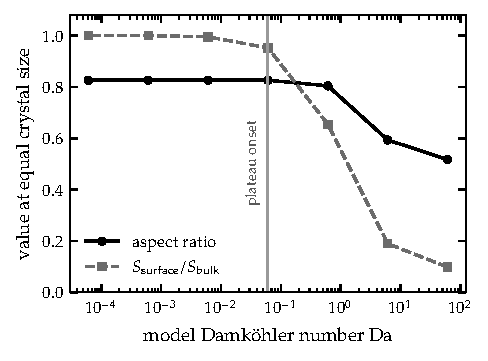
\includegraphics{fig_regime.pdf}
\caption{Shape of the same crystal (equivalent radius 30 cells, $200\times100$ grid) as a function of the model Damköhler number. Above Da $\approx0.6$ the crystal is low and rounded and its surface sees a fraction of the bulk supersaturation; below Da $\approx0.06$ nothing measured changes. Data from \code{docs/regime\_study.md}, section~1.}\label{fig:regime}
\end{figure}

On the plateau, dissolved silica and iron are uniform in the fluid. The \code{uniform} scheme exploits this: instead of solving transport, it recomputes uniform concentrations each step from the conserved totals. It agrees with the full implicit solution to \SI{0.28}{\percent} in area and is 86 times faster. The modes use it, with $\tau=\num{e4}$ at 200 cells across, scaled with the grid width so that the physical attachment speed is unchanged. The scheme cannot show depletion halos, so it is valid only for Da $\ll1$; every run states its model Da in \code{summary.json} and warns above the plateau.

\subsection{A readable reference and a fast twin}

The NumPy code is written for reading and is the definition of the physics. The Numba kernels are a second implementation of the same arithmetic, longer and commented line by line, and are trusted only because check~6 compares them with the reference: differences of about \num{e-15} after \num{3000} steps in three scenarios, with conservation preserved and results independent of the thread count. The fast path is about three times faster on one thread and five to six times with four to six threads. Beyond four threads large grids gain little, because the step is limited by memory traffic. The two backends agree to round-off, not bitwise, so exact replay needs the same backend.

\subsection{Choice of resolution}

The interface is about six cells wide, and its finite thickness rounds the apex of the crystal. The rounding vanishes only slowly as the grid is refined (Figure~\ref{fig:convergence}): the difference to the next finer grid shrinks by a factor of about 0.7 per doubling. The research grid is the smallest whose aspect ratio is within \SI{5}{\percent} of the 1600-cell value at a cost of about a minute; the explore grid is the cheapest that gives a recognisable crystal. Comparisons between explore runs are meaningful only at equal resolution.

\begin{figure}[ht]
\centering
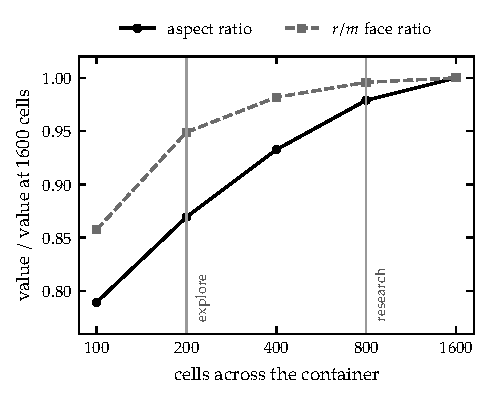
\includegraphics{fig_convergence.pdf}
\caption{Convergence of two shape measures with grid resolution, normalised by their values at 1600 cells across. The $r/m$ ratio converges quickly; the aspect ratio does not, because the interface rounds the apex. Vertical lines mark the two modes. Data from \code{docs/regime\_study.md}, section~3.}\label{fig:convergence}
\end{figure}

\subsection{Processes, not threads, for parallel work}

Ensembles and server jobs each run in a separate process started with \code{spawn}. A failed replica or job cannot corrupt the others, the server stays responsive during long computations, and each replica can use a single Numba thread without contention. Five replicas in parallel run about 3.7 times faster than one after another.

%======================================================================
\section{Model time and physical time}\label{sec:time}

Model time is reported together with two conversions, neither of which is a prediction of how long amethyst takes to grow. The diffusion time scale, $\Delta x^{2}/D$, is about \SI{10}{\second} per model unit for a \SI{0.1}{\milli\metre} cell; it is meaningful only for diffusion-limited runs. The kinetic conversion (\code{engine/time\_scaling.py}) applies in the surface-limited regime. It equates the model speed of the fastest face with the real front speed $V_\mathrm m\,k_+(T)\,(S-1)$, where $V_\mathrm m$ is the molar volume of quartz and $\log_{10}k_+=-0.7324-3705.12/T$ \citep{Takeno2000}. An optional pH term \citep{Palandri2004} raises $k_+$ about 3.16 times per pH unit in alkaline fluid and changes only this conversion.

The kinetic conversion gives \numrange{e7}{e9} years for crystals of millimetres to centimetres at \SIrange{15}{60}{\celsius}, while the host basalts are about \SI{135}{Myr} old \citep{Thiede2010} and the duration of the amethyst stage is not known. This tension is unresolved; candidate explanations are quantified in \code{docs/growth\_time.md}. The conversion assumes that the rate constant measured for quartz in neutral dilute solution applies to the fastest face and the geometric surface, and is uncertain by at least two orders of magnitude.

%======================================================================
\section{How correctness is checked}\label{sec:validation}

\code{scripts/validate.py} runs 14 checks (66 judged tests, about 35 minutes for \code{all}); each can be run alone by name. They fall into three groups. Checks against theory or a source: the isotropic front speed (check~1), Frank's construction for face positions and mirror symmetry when $r=z$ (check~2), the solubility curve against the printed equation (check~4), and the pH rate law against its source table (check~4b). Checks of bookkeeping: conservation of silica and iron, sector iron following the coefficients, reproducibility, exact replay of live sessions and ensembles, the server. Checks of numerics: resolution convergence (check~5), Numba against the reference (check~6), implicit and uniform schemes against the explicit one (check~6b). \code{docs/validation\_report.md} lists, for each check, what it shows and what it does not show.

No check compares the engine with a real crystal. A protocol and tool for that exist (\code{docs/observation\_comparison.md}) but have been exercised only with fictitious data.

%======================================================================
\section{Known limitations and open questions}\label{sec:limits}

The model is a single two-dimensional section of a three-dimensional crystal, in a closed container (unless renewal pulses are enabled) of pure water at constant or stepped temperature. Iron does not affect growth. The habit, the iron contrast between sectors and the replica spread follow from assumed values. Explore-mode shapes are qualitative. The model cannot produce hopper or skeletal faces even when driven far from the plateau, because it has no step-source kinetics; such facet destabilisation is a diffusion-limited effect not expected at geode Da in neutral fluid. The run warning threshold (Da $>0.06$ at 50 cells) does not cover the earliest plateau onset found (about \num{0.01}); lowering it is proposed but not applied.

Several literature values are marked \textsc{unverified} or \textsc{assumed} in the material file: the silica diffusivity above \SI{30}{\celsius}, the faceted phase-field formulation of \citet{Debierre2003} (summary only), the valid range of the solubility curve, and every face speed and iron coefficient. The most useful next steps are measured face-specific growth rates, measurements of a real amethyst section to compare against, and an independent constraint on the duration of geode growth.

%======================================================================
\section{Where to start reading}\label{sec:reading}

For the physics, read \code{engine/solution\_growth.py} top to bottom: its module docstring restates Eqs.~\eqref{eq:phasefield}--\eqref{eq:silica}, and its functions call \code{anisotropic\_phase\_field.py}, \code{anisotropy.py}, \code{silica\_transport.py} and \code{iron\_incorporation.py}. For the run machinery, read \code{simulation/modes.py} and then \code{simulation/controlled\_run.py}. Before changing any constant, read its entry in \code{materials/amethyst.yaml} and in \code{docs/parameter\_audit.md}. Before presenting any result, read \code{docs/validation\_report.md}. A first run and a check of the fast kernels:

\noindent\begin{minipage}{\linewidth}
\begin{lstlisting}[language=bash]
python scripts/run_live.py        # live window, explore size
python scripts/validate.py fast   # Numba vs reference (check 6)
\end{lstlisting}
\end{minipage}

\section*{Acknowledgements}
The author wrote some parts of the code; most of it was written by Claude (Anthropic) through Claude Code. The author's role was to define and validate the physical model, design the studies and checks, and review every result, sending the code back for fixes whenever something did not hold up.

\bibliographystyle{plainnat}
\begin{thebibliography}{9}
\bibitem[Cohen and Hassan(1974)]{Cohen1974}
A.~J. Cohen and F.~Hassan.
\newblock Ferrous and ferric ions in synthetic $\alpha$-quartz and natural amethyst.
\newblock \emph{American Mineralogist}, 59:719--728, 1974.

\bibitem[Debierre et~al.(2003)]{Debierre2003}
J.-M. Debierre, A.~Karma, F.~Celestini, and R.~Guérin.
\newblock Phase-field approach for faceted solidification.
\newblock \emph{Physical Review E}, 68:041604, 2003.

\bibitem[Palandri and Kharaka(2004)]{Palandri2004}
J.~L. Palandri and Y.~K. Kharaka.
\newblock A compilation of rate parameters of water--mineral interaction kinetics for application to geochemical modeling.
\newblock Open-File Report 2004-1068, U.S. Geological Survey, 2004. doi:10.3133/ofr20041068.

\bibitem[Rebreanu et~al.(2008)]{Rebreanu2008}
L.~Rebreanu, J.-P. Vanderborght, and L.~Chou.
\newblock The diffusion coefficient of dissolved silica revisited.
\newblock \emph{Marine Chemistry}, 112:230--233, 2008.

\bibitem[Rimstidt(1997)]{Rimstidt1997}
J.~D. Rimstidt.
\newblock Quartz solubility at low temperatures.
\newblock \emph{Geochimica et Cosmochimica Acta}, 61:2553--2558, 1997.

\bibitem[Takeno et~al.(2000)]{Takeno2000}
N.~Takeno, T.~Ishido, and J.~W. Pritchett.
\newblock Dissolution, transport and precipitation of silica in geothermal system.
\newblock In \emph{Proceedings of the World Geothermal Congress 2000}, pages 2943--2948, Kyushu--Tohoku, Japan, 2000.

\bibitem[Thiede and Vasconcelos(2010)]{Thiede2010}
D.~S. Thiede and P.~M. Vasconcelos.
\newblock Paraná flood basalts: rapid extrusion hypothesis confirmed by new $^{40}$Ar/$^{39}$Ar results.
\newblock \emph{Geology}, 38:747--750, 2010.
\end{thebibliography}

\end{document}
